\documentclass[xcolor=table]{beamer}

\usepackage{graphbox}       % For centre alignment of graphics
\usepackage{textcomp}       % Text companion fonts
\usepackage{listings}       % For code listings
\usepackage[]{inconsolata}

\setbeamertemplate{navigation symbols}{}
\setbeamertemplate{items}[circle]

\hyphenpenalty 4000 \sloppy


\lstset{
    language=VHDL,
    basicstyle=\scriptsize\ttfamily
}


\title{Notes on MBF FPGA Development}
\author{Michael Abbott}
\institute{FPGA Development Working Group}
\date{Tuesday 24\textsuperscript{th} April 2018}


\newcommand{\cc}{\cellcolor{green!60!blue!20}}

\begin{document}

\frame{\titlepage}


% ------------------------------------------------------------------------------
%
\begin{frame}{}

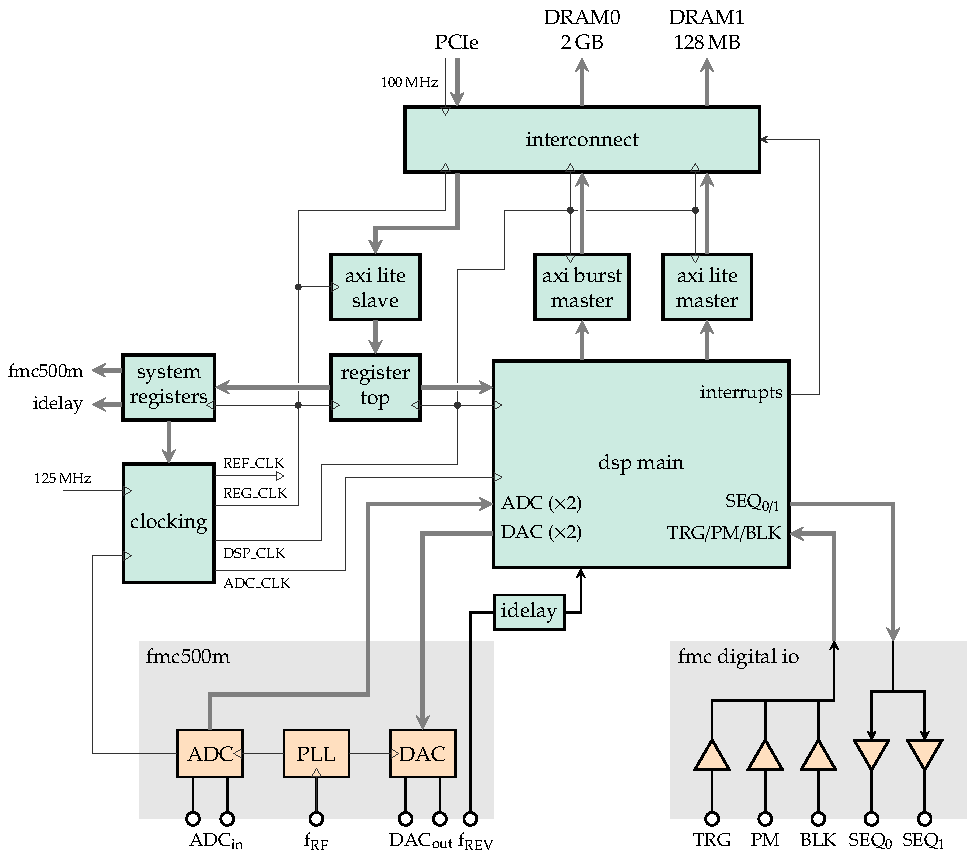
\includegraphics[width=\linewidth]{overview.pdf}

\end{frame}


% ------------------------------------------------------------------------------
%
\begin{frame}{Interconnect Overview}

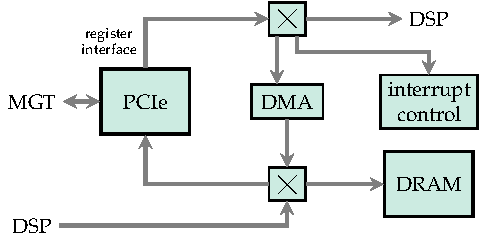
\includegraphics[width=0.8\linewidth]{interconnect.pdf}

Implemented using Xilinx Block Design tool, managed under source control as
Vivado generated \texttt{.tcl} script.

\end{frame}


% ------------------------------------------------------------------------------
%
\begin{frame}[fragile]{Register Interface: AXI $\to$ Internal}

\begin{lstlisting}
entity axi_lite_slave is
    port (
        clk_i : in std_logic;

        -- AXI-Lite read interface
        ... araddr_i rdata_o ready/valid
        -- AXI-Lite write interface
        ... awaddr_i wdata_i bresp_o ready/valid

        -- Internal read interface
        read_strobe_o : out std_logic;
        read_address_o : out unsigned;
        read_data_i : in std_logic_vector;
        read_ack_i : in std_logic;

        -- Internal write interface
        write_strobe_o : out std_logic;
        write_address_o : out unsigned;
        write_data_o : out std_logic_vector;
        write_ack_i : in std_logic
    );
end;
\end{lstlisting}

\end{frame}


% ------------------------------------------------------------------------------
%
\begin{frame}[fragile]{Register Multiplexer}

\begin{lstlisting}
entity register_mux is
    port (
        clk_i : in std_logic;

        -- Register write.
        write_strobe_i : in std_logic;
        write_address_i : in unsigned;
        write_data_i : in reg_data_t;
        write_ack_o : out std_logic;

        write_strobe_o : out std_logic_vector;
        write_data_o : out reg_data_t;
        write_ack_i : in std_logic_vector;

        -- Register read.
        read_strobe_i : in std_logic;
        read_address_i : in unsigned;
        read_data_o : out reg_data_t;
        read_ack_o : out std_logic := '0';

        read_data_i : in reg_data_array_t;
        read_strobe_o : out std_logic_vector;
        read_ack_i : in std_logic_vector
    );
end;
\end{lstlisting}

\end{frame}


% ------------------------------------------------------------------------------
%
\begin{frame}[fragile]{Register Timing}

\begin{lstlisting}
clk_i            |       |       |       |       |       |
                         ________________
read_address_o  XXXXXXXXX________________
                          _______
read_strobe_o   _________/       \_______
                         ________
read_data_i     XXXXXXXXX________XXXXXXXX
                         ________
read_ack_i      XXXXXXXXX        XXXXXXXX

                         ________________________________
read_address_o  XXXXXXXXX________________________________
                          _______
read_strobe_o   _________/       \_______________________
                                         ________
read_data_i     XXXXXXXXXXXXXXXXXXXXXXXXX________XXXXXXXX
                                          _______
read_ack_i      _________________________/       \_______
\end{lstlisting}

\end{frame}


% ------------------------------------------------------------------------------
%
\begin{frame}[fragile]{Register Definition File}

\begin{lstlisting}[language=]
# Used for top level hardware management
!SYS
    # Configuration information
    INFO        R
        # Number of taps in the ADC compensation filter
        .ADC_TAPS       8
        # Number of taps in the bunch-by-bunch feedback filter
        .BUNCH_TAPS     8
        # Number of taps in the DAC pre-emphasis filter
        .DAC_TAPS       8

    # System status register
    STATUS      R
        # Set if ADC clock is currently good
        .DSP_OK
        # Set if FMC500 VCXO power ok
        .VCXO_OK

    # Control register
    CONTROL     RW
        # FMC500 PLL clkin sel0
        .PLL_SEL0
        # FMC500 PLL clkin sel1
        .PLL_SEL1
\end{lstlisting}

\end{frame}


% ------------------------------------------------------------------------------
%
\begin{frame}[fragile]{Generated Files}

From register definition file can automatically generate:

\begin{itemize}
\item
    VHDL register offsets and bit field ranges.
\item
    C structure definitions, for example:
\begin{lstlisting}[language=C]
struct sys {
    struct sys_info {
        uint32_t adc_taps : 8;
        uint32_t bunch_taps : 8;
        uint32_t dac_taps : 8;
    } info;     // R
    struct sys_status {
        uint32_t dsp_ok : 1;
        uint32_t vcxo_ok : 1;
    } status;   // R
    struct sys_control {
        uint32_t pll_sel0 : 1;
        uint32_t pll_sel1 : 1;
    } control;  // RW
};
\end{lstlisting}
\item
    Documentation.
\end{itemize}
\end{frame}


% ------------------------------------------------------------------------------
%
\begin{frame}{DDR}

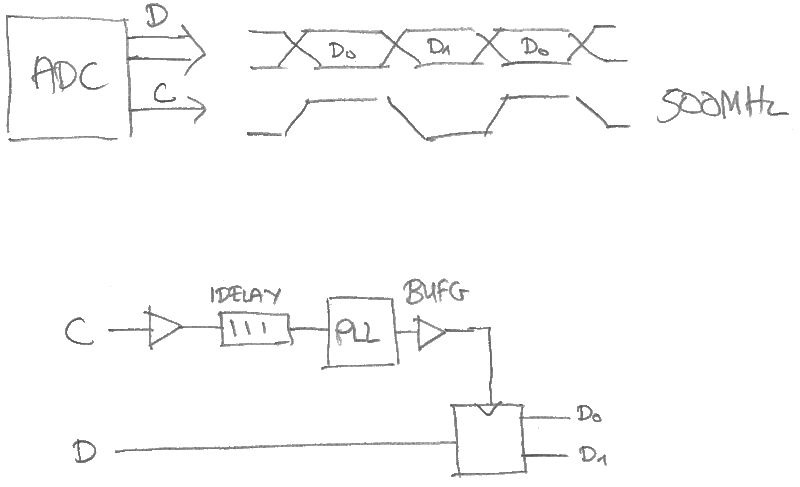
\includegraphics[width=\linewidth]{ddr.png}

\end{frame}


\end{document}
